

\documentclass[a4paper]{scrartcl}


% Mathematik-Pakete
\usepackage{amsmath}
\usepackage{amssymb}
\usepackage{amstext}
\usepackage{amsfonts}
\usepackage{mathrsfs}
\usepackage{paralist}
\usepackage[pdftex]{graphicx}
\usepackage{fancyhdr}
\usepackage{color}
\usepackage{hyperref}


%\usepackage[ansinew]{inputenc}
%\usepackage[T1]{fontenc}

\usepackage[utf8]{inputenc}
         
\usepackage[a4paper]{geometry}
\geometry{verbose,tmargin=1.5cm,lmargin=2cm,rmargin=2cm,bmargin=3cm,nohead}
\usepackage[ngerman]{babel}
\setlength{\parindent}{0cm}
\newcommand{\qed}{\begin{flushright}
$\blacksquare \dagger$ \end{flushright}}
\begin{document}
\pagestyle{fancy}
%\setlength{\footskip}{5mm}
\fancyhf{} 
\fancyfoot[C]{\thepage} %Seitennummer
\renewcommand{\headrulewidth}{0pt}
\renewcommand{\footrulewidth}{0.5pt}

%\twocolumn[
 \centerline{\LARGE \bf \textsf{MSE Tensor}} 
 \smallskip
\centerline{\Large \bf \textsf {Zusammenfassung}}
\medskip
  \centerline{\bf \textsf{dstrebel, s1bischo, sboller }}

 \smallskip \noindent\rule{\textwidth}{0.5pt}
\smallskip%]



% dies ist  noch einzubetten

Gradient eines Skalarfeldes: gibt die Richtung und Stärke des steilsten Anstiegs
eines Skalarfeldes an.
Skalarfeld $\Rightarrow$ Vektorfeld

Divergenz eines Vektorfeldes (Quellendichte eins Vektorfeldes): Gibt die Tendenz
eines Vektorfeldes an, von Punkten wegzufliessen (das gilt für positives
Vorzeichen; bei negativem Vorzeichen handelt es sich dementsprechend um die
Tendenz zu den Punkten hinzufliessen) Vektorfeld $\Rightarrow$ Skalarfeld

Rotation eines Vektorfeldes: Gibt die Tendenz eines Vektorfeldes an, um Punkte
zu rotieren; die Rotation eines Vektorfeldes ist ein Vektorfeld von
Pseudovektoren. Und zwar folgt aus dem Stokes’schen Integralsatz (siehe unten),
dass die Rotation die lokale Wirbeldichte eines Vektorfeldes beschreibt.

Quelle: http://de.wikipedia.org/wiki/Vektoranalysis



\section{Description of Physical Phenomena}
\subsection{Einheiten}

Mathe\\
$ [\lambda]=\frac{W}{mK} $\\
$ [\nabla]=\frac{1}{m} $\\

Wärme\\
$ [\rho]=\frac{kg}{m^3} (Dichte)$\\
$ [c_p]=\frac{J}{kgK} $\\
$ [m]=kg (Masse)$\\
$ [T]=K (Temperatur)$\\
$ [j_w]=\frac{W}{m^2} (Energieflussdichte)$\\
$ [I_W]=W (Waermefluss)$\\
$ [W]=\frac{J}{m^3} (???weiss nicht fuer was)$\\
$ [ \lambda ] = \frac{W}{mK} \text{(thermische Leitfähigkeit bzw. spez.  Wärmewiederstand)}????????? $\\
$ [ \sigma ]=??? ???)$\\
$ [ r ]=??? ???)$\\
\colorbox{red}{?????? prüfen} noch mehr? \\

Elektrotechnik\\
$ [Q]=C=As (el. Ladung)$\\
$ [F]=N=\frac{kg m}{s^2} (Kraft)$\\
$ [\dot W]=[P]=W=\frac{J}{s} (elektrische Leistung)$\\
$ [R] = \Omega = \frac{kg m^2}{A^2 s^3} (Widerstand/resistivity) $\\
$ [G] = S = \frac{1}{\Omega} \text{(elektrische Leitfähigkeit)}$\\
$ [\rho] = \Omega m (Spezifischer Widerstand)$\\
$ [\sigma] = \frac{1}{\Omega m} = \frac{S}{m} \text{(spezifische Leitfähigkeit,
Konduktivität)} $\\
$ [w]=\frac{kg}{ms^2} \colorbox{red}{nochmals kontrollieren!!!} $\\
$ [\vec E]=\frac{V}{m} = \frac{N}{C}$\\
$ [M]=Nm (Drehmoment)$\\
$ [\vec p]=Cm (Dipolmoment)$\\
$ [\rho]=\frac{C}{m^3} Ladungsdichte$\\
$ [D]=\frac{C}{m^2} (electrical Displacement)$\\
$ [\epsilon_0]= \frac{C^2}{Nm^2}=\frac{As}{Vm} (elektrische Feldkonstante)$\\
$ [\mu_0] = \frac{Vs}{Am} (magnetische Feldkonstante)$\\
$ [k] = \frac{Vm}{As} (Coulomb Konstante)$\\
$ [B]= T (Tesla) = \frac{kg}{As^2} = \frac{N}{Am} = \frac{Vs}{m^2} (magnetisches
Feld = magnetische Flussdichte)$\\
$ [H]= \frac{A}{m} (magnetische Feldstaerke)$\\
$ [U]= V = \frac{Nm}{As} (Spannung) $\\
$ [I]= A (Strom) $\\
$ [q]= C = As (Ladung)$\\
$ [m]= ??? (magnetic moment)$\\

Mechanik\\
$ [d]=\frac{N}{m} (Federkonstante)(spring constant)$\\
$ [E]=\frac{N}{m^2} (Federkonstante)(spring constant)$\\
$ [A]=A^2 (Flaeche)$\\
$ [F]=N (Kraft)$\\
$ [\sigma]=\frac{N}{m^2} (Spannung)(Stress)$\\
$ [l_0]=m (urspruengliche Laenge)$\\
$ [\delta l]=m (Laengenausdehnung)$\\
$ [\epsilon l]=- (Dehnung)(strain)$\\
$ [p]=Ns (Impuls)$\\



\subsection{SI-Einheiten}
$ J = \frac{kg m^2}{s^2} $\\

\subsection{Begriffe}
\begin{itemize}
\item extensive Grösse: wenn sich System verdoppelt verdoppelt sich auch die Eigenschaft z.B. Impuls, Volumen ...
\item intensive Grösse: wenn sich System verdoppelt verdoppelt sich Eigenschaft nicht z.B. Druck, Temperatur, ...
\end{itemize}


\subsection{Bilanzgleichungen}

\begin{tabular}{|c|c|c|c|c|}
\hline  & Stoffliche Grösse & Potential & Balance Equation uniform & Balance Equation distributed \\ 
\hline Charge Transport & Charge Q & el. Potential ??? & $\frac{dQ}{dt}=I_Q$ & $ \frac{\parallel p_Q}{\partial t}=-\nabla\cdot j_Q$ \\ 
\hline Heat Transport & thermal Energy W & Temperatur T & $\frac{\parallel W}{\partial t}= I_W+Q_W$ & $\frac{\parallel w}{\partial t}= -\nabla \cdot j_W+q_W$  \\ 
\hline Particle Transport & Partical number N & Particle density c & $\frac{dN}{dt}=I_N+Q_N$ & $\frac{dp}{dt}=-\nabla \cdot j_W +q_W$ \\ 
\hline Mechanics (Momentum Transport) & Momentum p & Velocity v  & $\frac{\partial p}{\partial t}=F$ & ?? \\ 
\hline 
\end{tabular} 

\subsection{Constitutive Laws}

\begin{tabular}{|c|c|c|c|}
\hline  & Storage Laws & Constitutive Laws & Source Rates and Sourcerate Densities \\
\hline Charge Transport & $j_Q=-\sigma \cdot \nabla ??? = \sigma \cdot E$ & & \\
 
\hline Heat Transport & $w=c_p \rho T$ & $j_W=-\lambda \cdot \nabla T$ &  \\ 
\hline Particle Transport (Diffusion) & c=c & $j_N=- D \cdot \nabla c_N$ &  \\ 
\hline Mechanics & $p=mv$ & $F_hook = - k \Delta u$ (Hook's Law) $F_visc=-C \eta \cdot v$ (Viscous Drag) &  \\ 
\hline 
\end{tabular} 




\section{Vektoranalysis und Integraltheorem}
\subsection{Nabla Operator}

\begin{align}
\nabla \: \mathrm{oder} \: \vec \nabla = \left (\frac\partial{\partial
x_1},\ldots, \frac\partial{\partial x_n}\right)
\end{align}
\subsection{Gradient}
Der Gradient ist ein mathematischer Operator, genauer ein Differentialoperator,
der auf ein \textbf{Skalarfeld} angewandt werden kann und in diesem Fall ein
Gradientenfeld genanntes \textbf{Vektorfeld} liefert, das die Änderungsrate d
Richtung der größten Änderung des Skalarfeldes angibt.

\begin{align}
\operatorname{grad}(f(x,y,z)) = \nabla f = \frac{{\partial f}}{{\partial x}} +
\frac{{\partial f}}{{\partial y}} + \frac{{\partial f}}{{\partial z}} = 
\begin{pmatrix} \frac{\partial f}{\partial x} \\ \frac{\partial f}{\partial
y} \\ \frac{\partial f}{\partial z} \end{pmatrix}
\end{align}

\subsection{Divergenz}
In der Mathematik ist die Divergenz ein Differentialoperator, der einem
\textbf{Vektorfeld} ein \textbf{Skalarfeld (Zahl)} zuordnet. Während bei einem
Vektorfeld jedem Punkt ein Vektor zugeordnet wird, wird bei einem Skalarfeld jedem Punkt ein Skalar, also
eine Zahl, zugeodnet. Interpretiert man das Vektorfeld als Strömungsfeld, so
gibt die Divergenz für jeden Raumpunkt an, wie viel mehr aus einer Umgebung
dieses Punkts hinausfließt als in sie hineinfließt. Mithilfe der Divergenz lässt
sich also herausfinden, ob und wo das Vektorfeld Quellen (Divergenz größer als
Null) oder Senken (Divergenz kleiner als Null) hat. Ist die Divergenz überall
gleich Null, so bezeichnet man das Feld als quellenfrei.

\begin{align}
\vec F = \begin{pmatrix} F_1 \\ F_2 \\ F_3 \end{pmatrix}
\end{align}

\begin{align}
\operatorname{div}\vec F = \nabla \cdot \vec F =
\frac{\partial}{\partial x_1}F_1 + \frac{\partial}{\partial x_2}F_2+ \frac{\partial}{\partial x_3}F_3
\end{align}

\subsection{Rotation (curl)}
Als Rotation bezeichnet man in der Vektoranalysis, einem Teilgebiet der
Mathematik, einen bestimmten Differentialoperator, der einem \textbf{Vektorfeld}
im dreidimensionalen euklidischen Raum mit Hilfe der Differentiation ein neues
\textbf{Vektorfeld} zuordnet. Handelt es sich beispielsweise um ein
Strömungsfeld, so gibt die Rotation für jeden Ort das Doppelte der Winkelgeschwindigkeit an, mit
der ein mitschwimmender Körper rotiert, also wie schnell und um welche Achse er
sich dreht. Dieser Zusammenhang ist namensgebend.

\begin{align}
\mathbf{\operatorname{rot}}\,\vec F(x,y,z) = \nabla\times \vec F =
\begin{pmatrix} \frac{\partial}{\partial x} \\ \frac{\partial}{\partial y} \\
\frac{\partial}{\partial z} \end{pmatrix} \times \begin{pmatrix} F_x\\ F_y\\ F_z
\end{pmatrix} = \begin{pmatrix} \frac{\partial F_z}{\partial y} - \frac{\partial
F_y}{\partial z} \\ \frac{\partial F_x}{\partial z} - \frac{\partial
F_z}{\partial x} \\ \frac{\partial F_y}{\partial x} - \frac{\partial
F_x}{\partial y} \end{pmatrix}
\end{align}

\begin{align}
\mathbf{\wedge = \times}
\end{align}


\subsection{Rechenregeln}
Es seien $\vec F$, $\vec G$ Vektorfelder und $U$, $V$ Skalarfelder.


\subsection{Gradient}

Gradient ist einfach gesagt die Ableitung in einer Richtung, wird dieser in mehreren Dimensionen angewendet schreibt man das Nabla Symbol $ \nabla $, nun einige Rechenregeln mit dem Gradient.

\begin{align}
\operatorname{grad}\,c=\vec{0}
\end{align}

\begin{align}
\operatorname{grad}\,(c\cdot u)=c\cdot\operatorname{grad}\,u
\end{align}

\begin{align}
\operatorname{grad}\,(u+v)=\operatorname{grad}\,u+\operatorname{grad}\,v
\end{align}

\begin{align}
\operatorname{grad}\,(u\, v) = u\ \operatorname{grad}\,v + v\ \operatorname{grad}\,u
\end{align}


\begin{align}
\label{eqn:ProduktregelEinesGradientMitPotenzen}
\operatorname{grad}\,(u^n) = n\, u^{n-1}\ \operatorname{grad}\,u \text{ für } n\neq 0
\end{align}


\subsection{andere}
\begin{align}
\operatorname{rot}(\operatorname{grad}U)=\nabla \times (\nabla U) = 0
\end{align}

\begin{align}
\operatorname{div}(\operatorname{rot}\vec{F}) = \nabla \cdot (\nabla \times
\vec F) = 0
\end{align}

\begin{align}
\operatorname{rot}(\operatorname{rot}\vec{F}) =
\operatorname{grad}(\operatorname{div}\vec{F}) -\Delta \vec{F}
\end{align}

\begin{align}
\operatorname{grad}(UV)=U\operatorname{grad}V+V\operatorname{grad}U
\end{align}

\begin{align}
\operatorname{grad}(\vec{F}\cdot \vec{G}) =
(\operatorname{grad}\vec{F})^{\operatorname t}\vec{G} + (\operatorname{grad}\vec{G})^{\operatorname t}\vec{F}
\end{align}

\begin{align}
\operatorname{div}(U\vec{F})=U\operatorname{div}\vec{F}+
\vec{F}\cdot\operatorname{grad}U
\end{align}

\begin{align}
\operatorname{div}(\vec{F}\times \vec{G})= \vec{G} \cdot
\operatorname{rot}\vec{F} -\vec{F}\cdot\operatorname{rot}\vec{G}
\end{align}

\begin{align}
\operatorname{rot}(U\vec{F})= U\operatorname{rot}\vec{F}
-\vec{F}\times\operatorname{grad}U\
\end{align}
\subsection{Satz von Gauss}
Der Integralsatz von  liefert den Zusammenhang zwischen einem Volumenintegral
über ein Volumen $V$, das von einem Feld $\vec F$ durchsetzt ist, und einem
Oberflächenintegral über die dieses Volumen umschliessende Fläche $A$. Die
Orientierung der Fläche sei so festgelegt, daß die Aussenseite die positive
Seite ist.

\begin{align}
\int_V \operatorname{div} \vec u \; \mathrm d^{(n)}V = \oint_{S} \vec u \cdot
\vec n\; \mathrm d^{(n-1)}A\,.
\end{align}
\subsection{Satz von Stokes}
Das Kurven- oder Linienintegral eines räumlichen Vektorfeldes $\vec u$ längs
einer geschlossenen Kurve $\partial F$ ist gleich dem Oberflächenintegral der
Rotation von $\vec u$ über eine beliebige Fläche $F$, die durch die Kurve
$\partial F$ berandet wird:

\begin{align}
 \int_{F} \operatorname{rot} \vec u \cdot d \vec A =
\oint_{\partial F} \vec u \cdot d \vec r
\end{align}


\section{Mathematical Basics}
\subsection{Grundlagen}


Einsteinnotation: $w_i=\sum_{j=1}^{3}A_ijv_j=A_ijv_j$
\\
Orthogonale Matrix ist, wenn gilt $MM^T=E$
\\


\subsection{Vector Algebra}
\begin{tabular}{|c|c|c|}
\hline  & Allgemein & in components \\ 
\hline Vector Addition & $w=u+v$ & $w_i=u_i+v_i$ \\ 
\hline Multiplication with a Scalar & $w=\alpha v$ & $w_i=\alpha v_i$ \\ 
\hline Scalar Product & $\alpha = v \cdot w $ & $\alpha = v_i w_i$ \\ 
\hline 
\end{tabular} 

\subsection{Tensor Algebra}
\begin{tabular}{|c|c|c|}
\hline  & Allgemein & in components \\ 
\hline Addition & $C=A+B$ & $C_{ij}=A_{ij}+B_{ij}$ \\ 
\hline Multiplication& $B=\alpha A$ & $B_{ij}=\alpha A_{ij}$ \\ 
\hline Product I & $C = a \otimes b $ & $C_{ij} = a_i b_j$ \\ 
\hline Product II& $C = A \otimes B $ & $C_{ijkl} = A_{ij} B_{kl}$ \\
\hline 
\end{tabular} 

\subsection{Tensorverjüngung}
\begin{tabular}{|c|c|l|}
\hline Allgemein & in components & Ausgedeutscht\\ 
\hline $c=A:B$ & $c=A_{ij}B_{ij}$ & $c = \sum\limits_{i=1}^{2}
\sum\limits_{j=1}^{2} A_{11} \cdot B_{11} + A_{12} \cdot B_{12} + A_{21} \cdot
B_{21} + A_{22} \cdot B_{22}$\\
& & c: Zahl, A \& B: 2nd rank Tensor
\\
\hline $B=\mathbb{D}:A$ & $B_{kl}=D_{klij}A_{ij}$ & \\
\hline $C=AB$ & $C_{ij}=A_{ik}B_{kj}$ & \\
& & C \& A \& B: 2nd rank Tensor (Entspricht Matrix Multiplikation)\\
\hline $w=Av$ & $w_i=A_{ij}v_{j}$ & \\
& & $w_i = \sum\limits_{j=1}^{2} a_{ij} \cdot v_j =
\begin{pmatrix}
A_{11} & A_{12}\\
A_{21} & A_{22}\\
\end{pmatrix} \begin{pmatrix} v_1 \\ v_2 \end{pmatrix}$ \\
& & (Entspricht Matrix Vektor Multiplikation)\\
\hline
$c = a b$ & $c = a_i b_i$ & $\vec{a} \cdot \vec{b} = a_i b_i =
\sum\limits_{i=1}^{2} a_i \cdot b_i = a_1 \cdot b_1 + a_2 \cdot b_2 + a_3 \cdot
b_3$\\
& & (Entspricht dem Skalarprodukt von 2 Vektoren)\\
\hline
\end{tabular} 
\\
\\
Bemerkung:
\begin{itemize}
\item c ist eine Zahl
\item A,B sind Tensoren zweiter Stufe
\item $\mathbb{D}$ ist ein Tensor vierter Stufe
\end{itemize} 


$ 
c = A_{ij}:B_{ij} 
$
$
=
\begin{pmatrix}
A_{11} & A_{12} \\ 
A_{21} & A_{22}
\end{pmatrix} 
$
:
$
\begin{pmatrix}
B_{11} & B_{12} \\ 
B_{21} & B_{22}
\end{pmatrix} 
$
$
=\varSigma_{i=1}^{2}\varSigma_{j=1}^{2}A_{ij}B_{ij}
$
$
=A_{11}B_{11}+A_{12}B_{12}+A_{21}B_{21}+A_{22}+B_{22}
$


\subsection{Bestimmen der Transformationsmatrix}
%Übung Exercise 3b) Aufgabe 3

Gegeben eine Matrix M... mit $det(A-\lambda E)$ die Eigenvektoren bestimmen und zusammensetzen ergibt die Transformationsmatrix R am Schluss Kontrollieren mit $M^{diag}=R \cdot R^T$



\subsection{Beispiel}
\subsubsection{Transformation 2nd Rank Tensor (Rotationsmatrix)}
$E'_{kl}=R_{ki}R_{lj}E_{ij}=R_{ki}E_{ij}R_{jl}^T$\\
$rotierteMatrix = Rotationsmatrix \cdot UrsprungsMatrix \cdot
Rotationsmatrix^{-1}$
\\
\\
Rotationsmatrix
\\
$R_x(\alpha) = \begin{pmatrix} 
1 &   0         & 0           \\
0 & \cos \alpha & -\sin \alpha \\
0 & \sin \alpha &  \cos \alpha
\end{pmatrix} $
\\
$R_y(\alpha) = \begin{pmatrix} 
\cos \alpha  & 0 & \sin \alpha \\
   0         & 1 &  0          \\
-\sin \alpha & 0 & \cos \alpha
\end{pmatrix} $
\\
$R_z(\alpha) = \begin{pmatrix} 
\cos \alpha & -\sin \alpha & 0 \\
\sin \alpha &  \cos \alpha & 0 \\            
   0        &  0           & 1
\end{pmatrix}$
\\

\subsubsection{2nd Rank Tensor Manipulation}

a) $\mathbf{C}=\mathbf{AB}$ $\Rightarrow$ $C_{ij}=A_{ik}B_{kj}$

Matrixmulitplikation weil die Dimension des resultierenden Tensors aus der
Anzahl Spalten des linken Tensors und der Anzahl Zeilen des Rechten Tensors
besteht. \qed

b) General heat conduction law $j_{th,k}=-\kappa_{kl}\frac{\partial
T}{\partial x_l}$ Prove that the isotropic law is recovered by using the
specific 2nd Rank Tensor $\kappa_{kl}=\kappa \delta_{kl}$

$K_{kl}$ Einsetzen. In diesem Fall ist das Korneckerdelta eine $1$. Deshalb
ergibt sich $-\kappa \frac{\partial T}{\partial x_k}$ \qed

c) Show that the 2nd Rank Unit Tensor $\mathbf{I}$ has the same form in each
coordinate system.$\Rightarrow$ Orthogonal

Transformation eines Einheitstensors: $\mathbf{I}'=R\mathbf{I}R'\Rightarrow$.
$I_{il}'=R_{ij}\delta_{jk}R_{kl}^T = R_{ij}R_{jl}^T=\delta_{il}=I_{il}$ \qed



d) Prove tr $\mathbf{E}=\mathbf{E : I}$
Component $\Rightarrow$ $E_{ij}\delta_{ij}=E_{ii}$ \qed

e) Prove every 2nd Rank can be written as symmetric and asymmetric tensor.

$\mathbf{A}=\frac{1}{2}\left(\mathbf{A} + \mathbf{A}^T\right)+
\frac{1}{2}\left(\mathbf{A}-\mathbf{A}^T\right) = \mathbf{A}$ \\
$\mathbf{A}=\left(\mathbf{A}_1^{sym}-\mathbf{A}_1^{sym}\right)=\left(\mathbf{A}_2^{sym}-\mathbf{A}_2^{sym}\right)$
\\
$0=\left(\mathbf{A}_1^{sym}-\mathbf{A}_2^{sym}\right)+\left(\mathbf{A}_1^{asym}-\mathbf{A}_2^{asym}\right)$
\\
$0=\mathbf{C}^{sym}+\mathbf{C}^{asym}$ $\Rightarrow$
$\mathbf{A}_1^{sym}=\mathbf{A}_2^{sym}$ $\Rightarrow$
$\mathbf{A}_1^{asym}=\mathbf{A}_2^{asym}$ \qed


f) \colorbox{red}{Kucksch du selber!, nicht realistisch!}




\subsection{Exercises of Chapter 3c)}

\subsubsection{4th Rank Tensor Manipulation}


$I_{ijkl}A_{kl}=\frac{1}{2}(\delta_{ik}\delta_{kl}+\delta_{il}\delta_{jk})A_{kl}=\frac{1}{2}(A_{ij}+A_{ji})=A_{ij}$
\\
\\
$ \mathbb{I} $ und $ \mathbb{E} $ sind unabhänig vom Koordinatensystem wenn diese isotrop sind

$ I'_{mnpq}=R_{mi}R_{nj}R_{pk}R_{ql}I_{ijkl} = \frac{1}{2}(R_{mi}\delta_{ik}R_{pk}R_{nj}\delta_{jl}R_{ql} + R_{mi}\delta_{il}R_{ql}R_{nj}\delta_{jk}R_{pk})= \frac{1}{2}(R_{mi}R^T_{ip}R_{nj}R^T_{jq}+R_{mi}R^T_{iq}R_{nj}R^T_{jp})= \frac{1}{2}(\delta_{mp}\delta_{mq}\delta_{np})=I_{mnpq} $ dasselbe gilt auch für $ E'_{mnpq}=E_{mnpq}$


\subsubsection{Engineering Notation}
\begin{itemize}
\item Weshalb gibt es den Faktor 2 bei $ \epsilon^{eng}=(\epsilon_{11},\epsilon_{22},\epsilon_{33},2\epsilon_{23},2\epsilon_{13},2\epsilon_{12}) $

???


\item Engineering notation von einem Einheitstensor zweiter Stufe
$ \textbf{I}^{eng}=(1,1,1,0,0,0) $


\item Notation von Tensoren 4 Stufe

\end{itemize}
$ \mathbb{I}^{eng}=
\begin{pmatrix}
1 & 0 & 0 & 0 & 0 & 0 \\ 
0 & 1 & 0 & 0 & 0 & 0 \\ 
0 & 0 & 1 & 0 & 0 & 0 \\ 
0 & 0 & 0 & \frac{1}{2} & 0 & 0 \\ 
0 & 0 & 0 & 0 & \frac{1}{2} & 0 \\ 
0 & 0 & 0 & 0 & 0 & \frac{1}{2}
\end{pmatrix} 
$

$
\mathbb{E}^{eng}=
\begin{pmatrix}
1 & 1 & 1 & 0 & 0 & 0 \\ 
1 & 1 & 1 & 0 & 0 & 0 \\ 
1 & 1 & 1 & 0 & 0 & 0 \\ 
0 & 0 & 0 & 0 & 0 & 0 \\ 
0 & 0 & 0 & 0 & 0 & 0 \\ 
0 & 0 & 0 & 0 & 0 & 0
\end{pmatrix} 
$

\section{Transport Phenomenas}
In diesem Kapitel werden anisotropische Transportphänomene betrachtet. Der
Begriff der Quadrik wird eingeführt. Im Fokus stehen thermische Leitfähigkeit,
elektrische Leitfähigkeit und Diffusion
\subsection{Theory}
\subsubsection{Quadrik}
Jeder symmetrischer Tensor 2-ter Stufe kann als Ellipsoid in drei dimensionalen
Raum dargestellt werden.

\begin{figure}[h]
\begin{center}
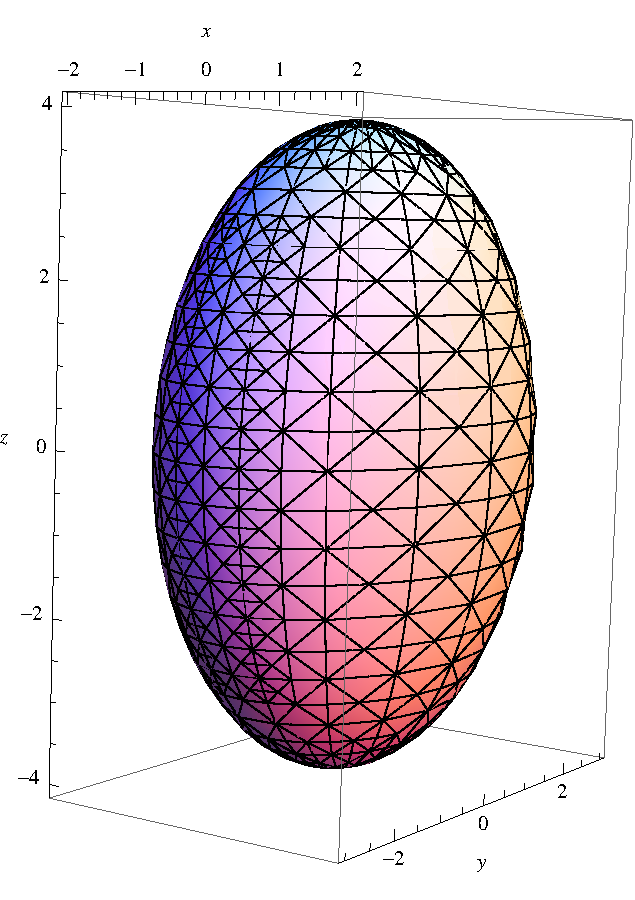
\includegraphics[scale=0.5]{images/ellipsoid.pdf}
\caption{Ellipsoid}
\label{fig:ellipsoid}
\end{center}
\end{figure}

Gegeben ist der symmtrische Tensor 2-ter Stufe:

\begin{align}
\sigma_{ij}=\begin{pmatrix}
\sigma_1 & 0 & 0 \\
0 & \sigma_2 & 0 \\
0 & 0 & \sigma_3 \\
\end{pmatrix}
\end{align}

Die quadrische Form kann folgendermassen erfüllt folgende Ellipsoidgleichung:

\begin{align}
\sigma_1x_1^2+\sigma_2x_2^2+\sigma_3x_3^2=1
\end{align}


Dabei entsprechen die Halbachsen:

\begin{align}
a=\frac{1}{\sqrt{\sigma_1}}; b=\frac{1}{\sqrt{\sigma_2}};
c=\frac{1}{\sqrt{\sigma_3}}
\end{align}

\begin{center}
Ellipse in 2D (Achsen $x_1$ und $x_2$):\\
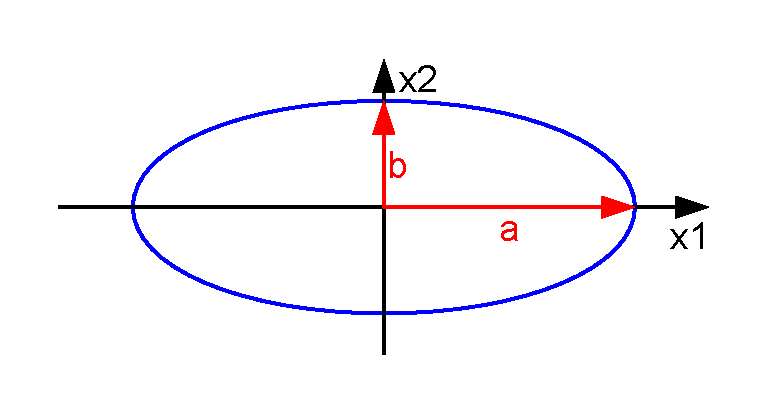
\includegraphics[scale=0.8]{images/quadrik_2d_ellipse.pdf}
\end{center}

\subsubsection{Thermal Conduction}
In isotropischen Medien ist die Wärmeleitung durch Fourier's Gesetz

\begin{align}
\mathbf{j}=-\lambda \nabla T
\end{align}

gegeben. In anistropischen Materialien ist die Wärmeleitung in Tensorform
gegeben:
\begin{align}
j_i=\lambda_{ij}\frac{\partial T}{\partial x_j}
\end{align}

Dieser Tensor ist gemäss Skript symmetrisch. Es gilt also
$\lambda_{ij}=\lambda_{ji}$

Dieser Tensor erfüllt folgende Quadrik:

\begin{align}
\lambda_1 x_1^2+\lambda_2 x_2^2+\lambda_3 x_3^2=1
\end{align}

Wobei $\lambda=\frac{1}{\rho}$ auch der Kehrwert des thermischen Widerstand ist.

\textbf{Special Case: Heat Flow across a flow plate} \\
Der Temperaturgradient ist parallel zur $x_1$ Richtung. $\frac{\partial
T}{\partial x_2}=0$ $\frac{\partial T}{\partial x_3}=0$

Demzufolge besteht der Tensor aus einem Eintrag:

\begin{align}
\lambda_{11}=\frac{j_1}{\partial T/ \partial x_1}
\end{align}

\textbf{Heat flow down a long rod}
Bei der Geometrie dieses Problems ist es besser mit dem thermischen Widerstand
zu arbeiten. Diesmal ist das Problem dreidimensional und durch folgende
Temperaturgradienten bestimmt.

\begin{align}
\frac{\partial T}{\partial x_1}=\rho_{11}j_1; \frac{\partial T}{\partial
x_2}=\rho_{12}j_1; \frac{\partial T}{\partial x_3}=\rho_{13}j_1
\end{align}

\subsubsection{Electrical Conduction}
Die fundamentale Gleichung ist das ohmsche Gesetz:

\begin{align}
j_i=-\sigma_{ij}\frac{\partial \phi}{\partial x_j}=\sigma_{ij}E_j
\end{align}

$j_i$ ist die Stromdichte, $\sigma_{ij}$ der elektrische Leitungstensor und
$E_j$ das elektrische Feld.

\subsubsection{Diffusion}
Bei der Diffusion gibt es ebenfalls eine Tensorvariante. Fick's law wird damit
verallgemeinert:

\begin{align}
j_i=-D_{ij}\frac{\partial c}{\partial x_j}
\end{align}

\subsection{Beispiele}
\subsubsection{2D Carbon Plate Thermal Conduction}

a) Conductivity Tensor of the problem

\begin{align}
k_{ij}=\begin{pmatrix}
50 & 0 & 0 \\
0 & 250 & 0 \\
0 & 0 & 250 
\end{pmatrix}
\end{align}
\qed
\begin{align}
a = \frac{1}{\sqrt{\sigma_1}} = \frac{1}{\sqrt{50}} \text{ und } b =
\frac{1}{\sqrt{\sigma_2}} = \frac{1}{\sqrt{250}}
\end{align}

\begin{center}
Ellipse Conductivity Tensor Quadrik:\\
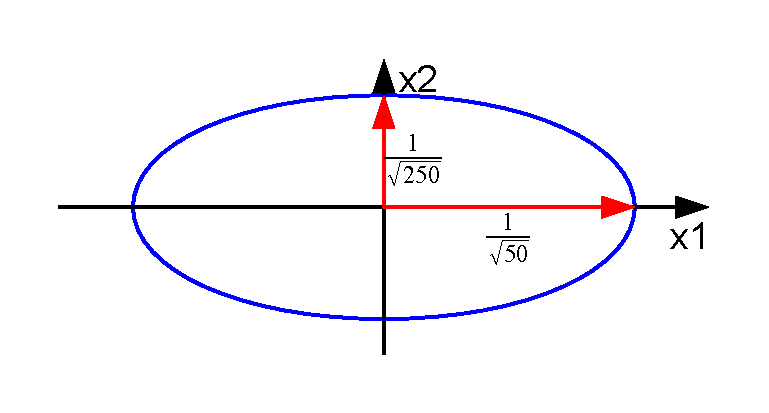
\includegraphics[scale=0.8]{images/quadrik_2d_ellipse_uebung.pdf}
\end{center}


b) Transformation $30^\circ$
\begin{align}
k_{ij}'=RkR^{T}
\end{align}

\begin{align}
\phi=+30^\circ
\end{align}

\begin{align}
k_{ij}'=\begin{pmatrix}
\cos{\phi} & -\sin{\phi} & 0 \\
\sin{\phi} & \cos{\phi} & 0 \\
0 & 0 & 1
\end{pmatrix}
\cdot
\begin{pmatrix}
50 & 0 & 0 \\
0 & 250 & 0 \\
0 & 0 & 250 
\end{pmatrix}
\cdot
\begin{pmatrix}
\cos{\phi} & \sin{\phi} & 0 \\
-\sin{\phi} & \cos{\phi} & 0 \\
0 & 0 & 1
\end{pmatrix}
\end{align}

\begin{align}
k_{ij}'=\begin{pmatrix}
100 & -86.60 & 0 \\
-86.60 & 200 & 0 \\
0 & 0 & 250
\end{pmatrix}
\end{align}
\qed

c) Heatflow in x1 Direction, $30^\circ$ Rotated Material

Alle Ableitungen bis auf $\frac{\partial T}{\partial x1}=a$ sind 0


\begin{align}
j_i=-k_{ij} \frac{\partial T}{\partial x_j}
\end{align}

\begin{align}
\vec{j}=\begin{pmatrix}
100 \\
-86.6 \\
0
\end{pmatrix}
\cdot -a
\end{align}

\qed
d) Ellipsoid

\begin{center}
Gedrehter Tensor (nicht im Hauptachsensystem):\\
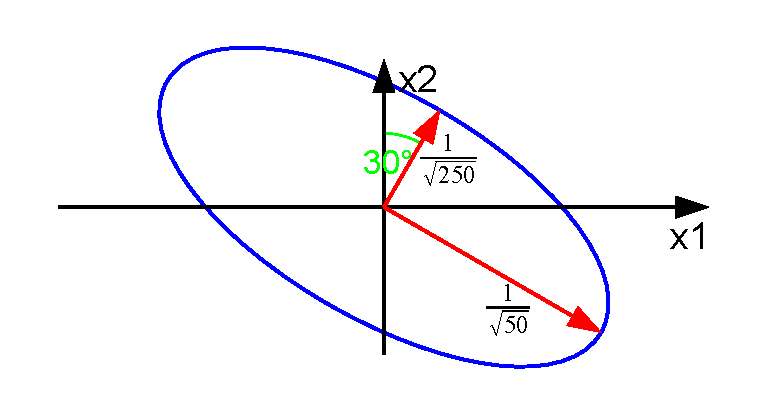
\includegraphics[scale=0.8]{images/quadrik_2d_ellipse_uebung_rotation.pdf}
\end{center}

e) Determine the resistivity $r_{12}$

\begin{align}
r_{ij}=\frac{1}{k_{ij}}=\begin{pmatrix}
\frac{1}{k_{11}} & 0 & 0 \\
0 & \frac{1}{k_{22}} & 0 \\
0 & 0 & \frac{1}{k_{33}}
\end{pmatrix}
\end{align}

\begin{align}
r_{ij}'=Rr_{ij}R^{T} = \begin{pmatrix}
16 & 6.9 & 0 \\
6.9 & 8 & 0 \\
0 & 0 & 4
\end{pmatrix}
10^{-3}[\frac{mK}{W}] 
\end{align}
\qed




\subsubsection{Eletrical Tin}
Write down the conductivity Tensor:

\begin{align}
\sigma_{ij} = \frac{1}{\rho_{ij}}= \begin{pmatrix}
101 & 0 & 0 \\
0 & 101 & 0 \\
0 & 0 & 69.9 
\end{pmatrix}
10^5 Sm
\end{align}

a) Calculate the magnitude and the direction of the current density

\begin{align}
j_i=\sigma_{ij}E_j
\end{align}

Multiplizieren mit Feld. Danach Vektorbetrag und Winkel berechnen. :-)

Winkel:

\begin{align}
\tan{\alpha}=\frac{Gegenkathete}{Ankathete}
\end{align}
\qed

\section{Elasticity}
\subsection{Elasticity in 1D}
\subsubsection{Implussfluss}
Generell folgen Elastizitätsprobleme Hook's Law:

\begin{align}
F=d \cdot \Delta u
\end{align}
Dabei ist $d$ die Federkonstante (materialabhängig) und $\Delta u$ die
Längenänderung des betrachteten Körpers.

Im mehrdimensionalen Fall bietet sich das Rechnen mit Flüssen an. Im
Elastizitätsfall ist dies der Impulsfluss. Über die Definition des Impulses
nach:

\begin{align}
p = m \cdot v
\end{align}

Daraus ergibt sich der Impulsfluss als:

\begin{align}
[J_p]=\frac{kg \cdot \frac{m}{s}}{s} \equiv N
\end{align}

also Kraft.

Impuls kann nur von einem Objekt auf ein anderes übertragen werden.
Gespeicherter Impuls setzt deshalb ein Objekt in Bewegung. (Beispiel
Tennisball: Ein in Bewegung gesetzter, fliegender Tennisball enthält den Impuls
$p=m \cdot v$)

Im Fall eines deformierten und an einer Wand befestigten Gummibandes kann man
sich den Impulsfluss folgendermassen vorstellen: Obwohl sich nichts bewegt,
fliesst der Impulsfluss nach der obigen Definition durch das Gummiband in die
Wand hinein (Energieerhaltung). Sobald das Band von der Wand gelöst wird, setzt
es sich in Bewegung $\Rightarrow$ Der Impuls ist nun im Band gespeichert. 

Es ist möglich an jeder Position des Bandes ($0<x_0<L$) den Impulsfluss zu
messen. An jedem $x_0$ muss die Kraft F aufgewendet werden um das Band in
gedehnten Zustand zu halten.

\subsubsection{Mechanical Stress \& Impulsflussdichte}
Wie jeder Fluss kann dieser als Flussdichte ausgedrückt werden. Definition der
Flussdichte ist:


\begin{align}
j_p = \frac{J_p}{A} \Rightarrow [\sigma_{11}]= \frac{N}{m^2} = Pa
\end{align}

Das Mechanische Stressfeld ist als negative Impulsflussdichte definiert:
 
\begin{align}
\sigma_{11}=- \frac{J_p}{A} \Rightarrow [\sigma_{11}]= \frac{N}{m^2} = Pa
\end{align}

Integriert man über dieses mechanische Stressfeld:

\begin{align}
F=\int_A dA \cdot \sigma_{11}
\end{align}
so erhält man \flqq Cutting Force\frqq. 
\subsubsection{1D-Equations}

Um 1-D Elastizitätsprobleme zu lösen, benötigen wir drei Gleichungen:

Balance:
\begin{align}
0=\frac{\partial \sigma_{11}}{\partial x}+\rho g_1
\end{align}

Material law:
\begin{align}
\epsilon_{11}=\frac{\partial u(x)}{\partial x} \\
\sigma_{11}= E \cdot \epsilon_{11}
\end{align}

Boundary conditions:
\begin{align}
\sigma_{11}(L)=\frac{F}{A}, u(0)=0
\end{align}

$u(x)$ wird als \flqq Displacement Field\frqq{} bezeichnet. Definiert ist diese
Funktion:

\begin{align}
u(x)=\Delta u \cdot \frac{x}{L}
\end{align}

$\Rightarrow$ Siehe Beispiele
\subsubsection{Elasticity in 3D}
Generell lässt sich die Gleichung analog zur Ladungsgleichung. Es gibt aber
Unterschiede: Der Impuls ist eine vektorielle Grösse. Als Konsequenz wird
$\sigma$ zu einem Tensor zweiter Stufe:

\begin{align}
\sigma = \begin{pmatrix}
\sigma_{11} & \sigma_{12} & \sigma_{13} \\
\sigma_{21} & \sigma_{22} & \sigma_{23} \\
\sigma_{31} & \sigma_{32} & \sigma_{33} 
\end{pmatrix}
\end{align}

Möchte man nun die Impulsbilanz vektoriell in x-Richtung aufstellen ergibt sich
(1D-vektoriell):

\begin{align}
0=\frac{\partial \sigma_{1k}}{\partial x_k}
\end{align}

Weiter verallgmemeinert ergibt sich im 3D Fall:

\begin{align}
0=\frac{\partial \sigma_{ik}}{\partial x_k}
\end{align}

Wird zusätzlich das Gravitationsfeld berücksichtigt, ergibt sich noch folgende
Verallgemeinerung:

\begin{align}
0=\frac{\partial \sigma_{ik}}{\partial x_k} + \rho g_i
\end{align}

\subsubsection{Eigenschaften des Stress Tensors}
Um sich den Stresstensor intuitiv vorzustellen, machen wir folgende Annahme:
Wir betrachten einen Hexaeder (beliebiger Körper mit sechs Flächen). Externe
Kräfte wirken auf diesen Körper. An jeder der 6 Flächen haben wir eine
resultierende Kraft $\vec F^\alpha$
\subsection{Beispiel}

\begin{minipage}{3cm}
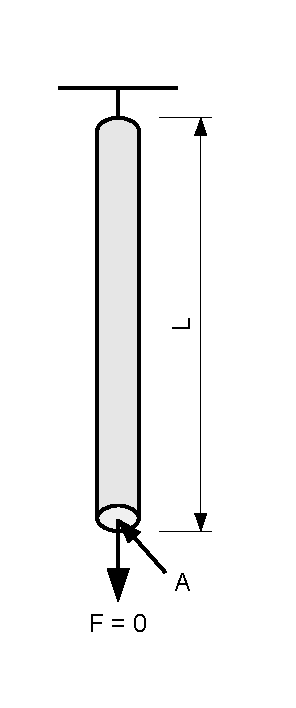
\includegraphics[scale=0.6]{images/elasticity_robe.pdf}
\end{minipage}
\hfill
\begin{minipage}{14cm}
Balance equation: $0 = \frac{\partial \sigma_{11}}{\partial x} + \rho g_1$\\
Material law: $\epsilon_{11} = \frac{\partial u(x)}{\partial x}$ with
$\sigma_{11} = E \cdot \epsilon_{11}$\\
Boundary conditions: $\sigma_{11} (L) = \frac{F}{A}$, $u(0)= 0$\\

DGL aufstellen: $\frac{\partial \sigma (x)}{\partial x} = - \rho g$ $\mid$ $\int
dx$\\
DGL lösen: $\sigma (x) = - \rho g x + \sigma_0$\\
Boundary Conditions bei L: $\sigma (L) = \frac{F}{A} = \frac{0}{A} = 0$\\
BC in DGL einsetzen: $\sigma (L) = - \rho g L + \sigma_0 = 0$\\
Auflösen: $\sigma_0 = \rho g L$\\
In DGL einsetzen: $\sigma (x) = - \rho g x + \rho g L = \rho g (L-x)$\\
Material law: $\epsilon (x) = \frac{\rho g}{E} (L-x)$\\
Aus Material law: $\frac{\partial u(x)}{\partial x} = \epsilon (x) = \frac{\rho
g}{E} (L-x)$ $\mid$ $\int dx$\\
Deformation: $u(x) - u(0) = \int\limits_{0}^{x} \epsilon(x) dx =
\int\limits_{0}^{x} \frac{\rho g}{E} (L-x) dx = \frac{\rho g}{E} (x \cdot L -
\frac{1}{2} \cdot x^2) = \frac{\rho g}{E} \cdot x(L-\frac{x}{2})$, wobei $u(0) =
0$\\
\colorbox{red}{Was zum Teufel passiert mit dem
Integral?????? -> kei Plan}$\int\limits_{0}^{x} x \cdot dx$
\end{minipage}
\textbf{Maximaler Stress} tritt an der Aufhängung an Punkt $x = 0$ auf:\\
$\sigma(0) = - \rho g (L-x) = \rho g L = \frac{m \cdot g}{A}$\\
Einheitenkontrolle: $[\rho \cdot g \cdot L] = \frac{kg}{m^3} \cdot
\frac{m}{s^2} \cdot m = \frac{kg}{m \cdot s^2}$\\
$[m \cdot g \cdot \frac{1}{A}] = kg \cdot \frac{m}{s^2} \cdot \frac{1}{m^2} =
\frac{kg}{m \cdot s^2}$\\
\subsubsection{Nochmals das gleiche mit Gewicht}
$F \neq 0$ $\to$ $\sigma(L) = \frac{M
g}{A}$\\
DGL aufstellen: $\frac{\partial \sigma (x)}{\partial x} = - \rho g$ $\mid$
$\int dx$\\
DGL lösen: $\sigma (x) = - \rho g x + \sigma_0$\\
Boundary Conditions bei L: $\sigma (L) = \frac{F}{A} = \frac{M g}{A}$\\
BC in DGL einsetzen: $\sigma (L) = - \rho g L + \sigma_0 = \frac{M g}{A}$\\
Auflösen: $\sigma_0 = \rho g L + \frac{M
g}{A}$\\
In DGL einsetzen: $\sigma (x) = - \rho g x + \rho g L + \frac{M g}{A}= \rho g
(L-x) + \frac{M g}{A}$\\
Material law: $\epsilon (x) = \frac{\rho g}{E} (L-x) + \frac{M g}{E A}$\\
Aus Material law: $\frac{\partial u(x)}{\partial x} = \epsilon (x) = \frac{\rho
g}{E} (L-x) + \frac{M g}{E A} =  \frac{g}{E} (\rho L + \frac{M}{A} - \rho x) $
$\mid$ $\int dx$\\
Deformation: $u(x) - u(0) = \int\limits_{0}^{x} \epsilon(x) dx =
\int\limits_{0}^{x} \frac{g}{E} (\rho L + \frac{M}{A} - \rho x) dx =
\frac{g}{E} \cdot x \left( \left( L \rho + \frac{M}{A} \right) -
\frac{x \rho}{2}\right)$, wobei $u(0) = 0$\\

\subsubsection{Spring Constant (Federkonstante)}
Definition Federkonstante: $F = d \cdot \Delta u $\\
$\sigma = \frac{F}{A}$ $\Rightarrow$ (siehe Übung oben) $u(x) = \frac{F}{A E}
x$\\
Für 1D und isotrop über ganzes Gummiband: $x = L$\\
$\Delta u = \frac{F L}{A E}$\\
Aus $F = d \cdot \Delta u $ ergibt sich: $d = \frac{A E}{L}$

\subsection{Beispiel Teil 2 (Strain, Stress, \ldots)}

\subsubsection{Pure Shear Stress}

\textbf{Momentum flux}\\
\begin{minipage}{6cm}
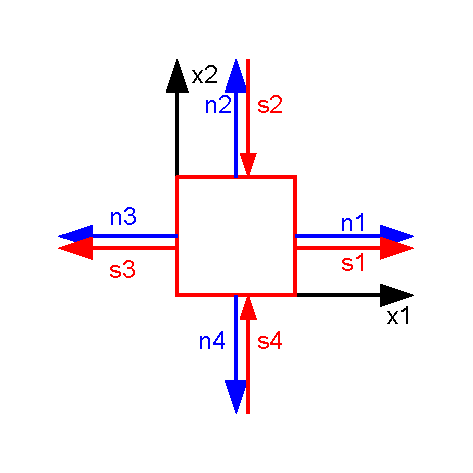
\includegraphics[scale=0.8]{images/pure_shear_stress_1.pdf}
\end{minipage}
\hfill
\begin{minipage}{14cm}
Gegeben: $\sigma = \begin{pmatrix}
s & 0 & 0\\
0 & -s & 0\\
0 & 0 & 0\\
\end{pmatrix} $\\
cutting forces on each face:\\
$s_1 = \sigma \vec n_1 = \begin{pmatrix}
s & 0\\
0 & -s\\
\end{pmatrix} \begin{pmatrix}
1\\
0\\
\end{pmatrix} = \begin{pmatrix}
s\\
0\\
\end{pmatrix}$\\

$s_2 = \sigma \vec n_2 = \begin{pmatrix}
s & 0\\
0 & -s\\
\end{pmatrix} \begin{pmatrix}
0\\
1\\
\end{pmatrix} = \begin{pmatrix}
0\\
-s\\
\end{pmatrix}$\\

$s_3 = \sigma \vec n_3 = \begin{pmatrix}
s & 0\\
0 & -s\\
\end{pmatrix} \begin{pmatrix}
-1\\
0\\
\end{pmatrix} = \begin{pmatrix}
-s\\
0\\
\end{pmatrix}$\\

$s_4 = \sigma \vec n_4 = \begin{pmatrix}
s & 0\\
0 & -s\\
\end{pmatrix} \begin{pmatrix}
0\\
-1\\
\end{pmatrix} = \begin{pmatrix}
0\\
s\\
\end{pmatrix}$

\end{minipage}

\textbf{Transform}\\
Transformation as usual:
\begin{align}
\sigma'_{kl}=R_{ki}R_{lj}\sigma_{ij}=R_{ki}\sigma_{ij}R_{jl}^T \\
R_{kl}=\begin{pmatrix} 
\cos \alpha & -\sin \alpha & 0 \\
\sin \alpha &  \cos \alpha & 0 \\            
   0        &  0           & 1
\end{pmatrix}
\end{align}

Resultat:

\begin{align}
\sigma'_{kl}=\begin{pmatrix}
0 & s & 0 \\
s & 0 & 0 \\
0 & 0 & 0
\end{pmatrix}
\end{align}

\textbf{Trace}\\

\begin{align}
\operatorname{tr}\sigma_{kl}=0 \\
\operatorname{tr}\sigma'_{kl}=0 
\end{align}

$\Rightarrow$ Pure Shear Stress
\qed
\subsubsection{Stress in the Principal Axis System}
Gegeben:
\begin{align}
\sigma=\begin{pmatrix}
-\frac{2}{25} & 0 & \frac{36}{25} \\
0 & 3 & 0 \\
\frac{36}{25}& 0 & -\frac{23}{25}
\end{pmatrix}
\end{align}

Find Eigenvalues:

\begin{align}
\operatorname{eig}(\sigma)=\left(1,-2, 3\right) \operatorname{or}
\left(1,3,-2\right)
\end{align}
\colorbox{red}{Unbedingt Fragen, wichtig oder nicht???}

Resultat:

\begin{align}
\sigma'=\begin{pmatrix}
1 & 0 & 0 \\
0 & 3 & 0 \\
0 & 0 & -2
\end{pmatrix}
\end{align}
\textbf{Transformation}\\

\textbf{Decompose}\\

\subsubsection{Deformation Strain State}



\section{Electrodynamics}

\colorbox{red}{Skriptzusammenfassung...}

$ \vec{p}=q\cdot\vec{d} $


\subsection{Sonstiges}



\subsubsection{E-Feld}

In der Abbildung \ref{fig:E-Feld} ist ein homogenes Elektisches Feld (E-Feld) gezeichnet.

\begin{figure}[h!]
\begin{center}
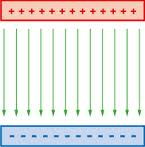
\includegraphics[scale=0.5]{images/E-Feld.jpg}
\caption{E-Feld}
\label{fig:E-Feld}
\end{center}
\end{figure}

In der Abbildung \ref{fig:E-Feldstaerke} ist ebenfalls ein E-Feld $ \vec{E} $ abgebildet, wobei hier die Länge der Vektoren gleich der elektrischen Feldstärke entspricht, diese ist in diesem Fall nicht homogen.

\begin{figure}[h!]
\begin{center}
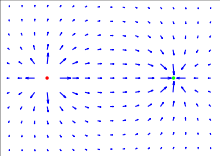
\includegraphics[scale=0.5]{images/E-Feldstaerke.png}
\caption{E-Feldstärke entspricht der Länge der Vektoren}
\label{fig:E-Feldstaerke}
\end{center}
\end{figure}



\subsubsection{B-Feld (Magnetfeld)}
$B = \mu \cdot H$\\
\begin{figure}[h!]
\begin{center}
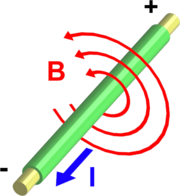
\includegraphics[scale=0.5]{images/B-Feld.png}
\caption{B-Feld}
\label{fig:B-Feld}
\end{center}
\end{figure}

\subsubsection{Anwendung}

\begin{center}
\begin{tabular}{|c|c|}

\hline Strom & Daumen \\ 
\hline B-Feld & Zeigefinger \\ 
\hline Kraft & Mittelfinger \\ 
\hline 

\end{tabular} 
\end{center}


\begin{center}
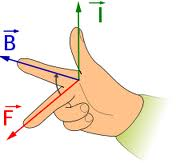
\includegraphics[scale=0.5]{images/handregel.jpg}
\end{center}

\begin{center}
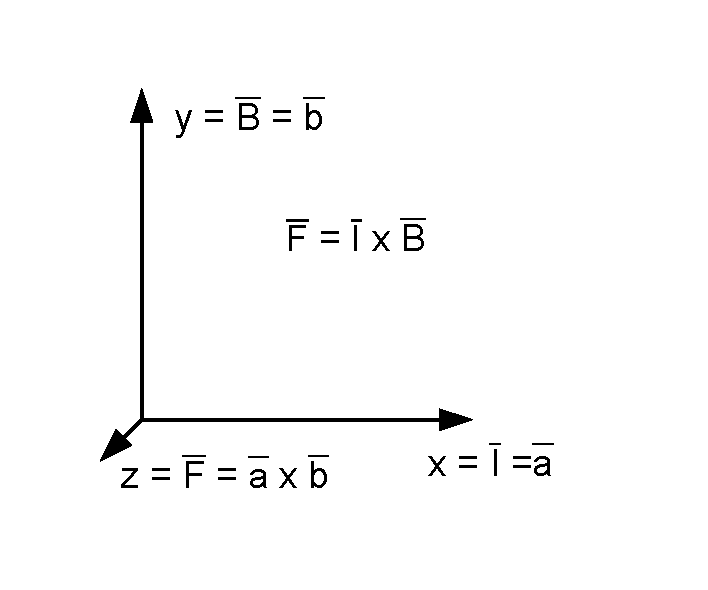
\includegraphics[scale=0.5]{images/kreuzprodukt.pdf}
\label{fig:kreuzprodukt}
\end{center}


\begin{figure}[h!]
\begin{center}
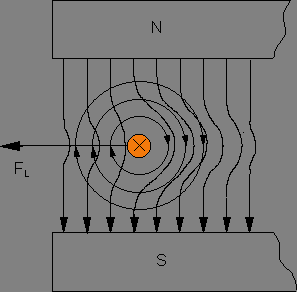
\includegraphics[scale=0.5]{images/DrahtZwischenPolen.png}
\caption{Draht zwischen Polen}
\label{fig:DrahtZwischenPolen}
\end{center}
\end{figure}


\subsection{Exercise}
\subsubsection{Useful formulas}

Gradient von $ (\frac{1}{r}) $  with $ r=\sqrt{x^2+y^2+z^2} $

Anwenden von der Produktregel eines Gradient, siehe Formel \ref{eqn:ProduktregelEinesGradientMitPotenzen} auf Seite \pageref{eqn:ProduktregelEinesGradientMitPotenzen}

$ \nabla(\frac{1}{r}) = -\frac{\vec{r}}{r^3}$
\\
$ \nabla(\frac{1}{r^2}) = -2\frac{\vec{r}}{r^4}$
\\
$ \nabla(\frac{1}{r^3}) = -3\frac{\vec{r}}{r^5}$

\subsubsection{The electrical field}

Info A\\
Berechnung von curl von einer Punktladung.\\ 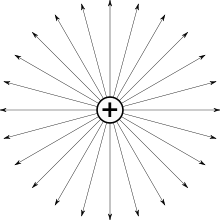
\includegraphics[scale=0.2]{images/punktladung.png}
\label{fig:Punktladung}

$ \vec{E}(\vec{r})=\frac{q}{4\Pi\epsilon_0}\frac{\vec{r}}{r^3}\sim \frac{\vec{r}}{r^3} $
\\
$ \vec{\nabla}\times\vec{E}\approx\vec{\nabla}\times(\frac{\vec{r}}{\vec{r^3}})=\frac{\vec{1}}{r^3}(\vec{\nabla}\times\vec{r})+\vec{r}\times(\vec{\nabla}(\frac{1}{r^3}))=-\frac{3}{r^5}(\vec{r}\times\vec{r})=0 $

Info B\\
$ k=\frac{1}{4\pi\epsilon_0} $

Info C\\


Info D\\

\subsubsection{Polar Molecules (Torque and force)}

torque on molecule by an electrical field\\

$ \vec{F}=q\cdot\vec{E}$\\

$ \vec{M}=\vec{r}\cdot\vec{F}$\\

$ \vec{M}=\vec{p}\times\vec{E}$\\

Non uniform E-Field\\

\begin{align}
\vec F = \begin{pmatrix}
P_x \frac{\partial E_x}{\partial x} + P_y \frac{\partial E_x}{\partial y} + P_z
\frac{\partial E_x}{\partial z}\\
P_x \frac{\partial E_y}{\partial x} + P_y \frac{\partial E_y}{\partial y} + P_z
\frac{\partial E_y}{\partial z}\\
P_x \frac{\partial E_z}{\partial x} + P_y \frac{\partial E_z}{\partial y} + P_z
\frac{\partial E_z}{\partial z}\\
\end{pmatrix}
= \operatorname{grad} (\vec E) \cdot \vec p
\end{align}

\subsubsection{Maxwell's equation}
\begin{itemize}

\item Die Quelle des E-Feldes ist die Ladung. Der elektrische Fluss über die
geschlossene Oberfläche entspricht der eingeschlossenen Ladung.\\
$ \vec \nabla \vec D = \rho \rightarrow \oint_{\partial V} \vec D \cdot \vec n
dA = Q$\\
$\vec D = \epsilon_0 \vec E$\\

\begin{center}
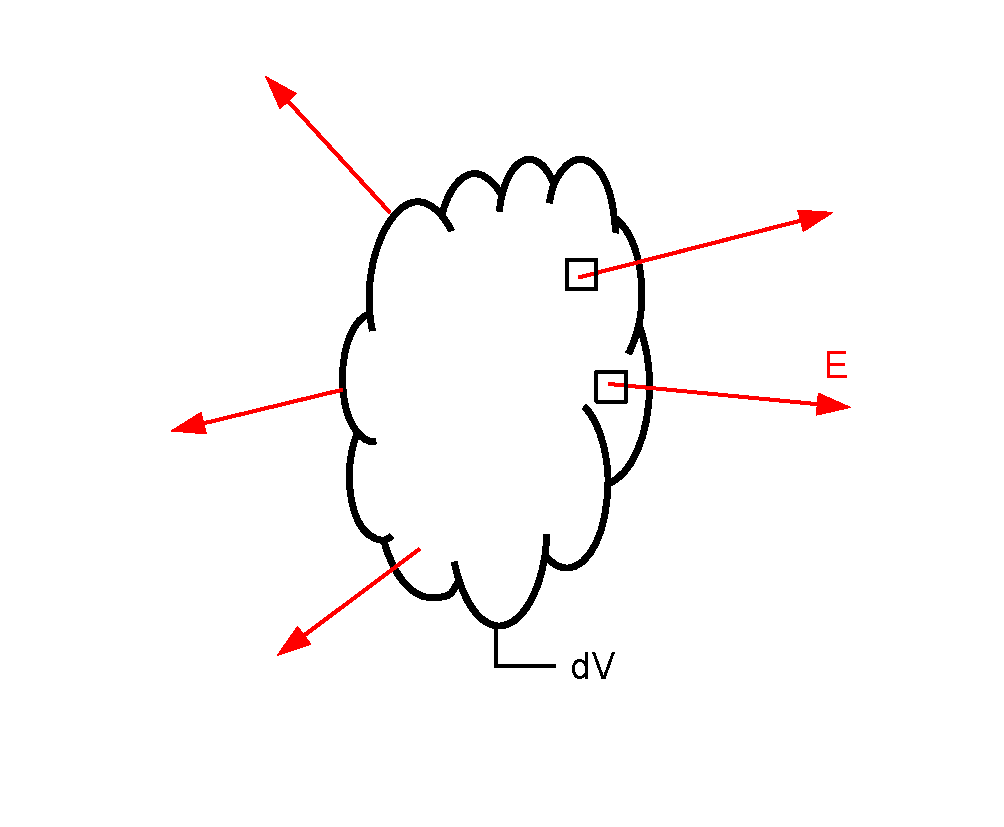
\includegraphics[scale=0.5]{images/maxwell_1.pdf}
\end{center}

\item Es existieren keine magnetische Monopole im Volumen. Magnetische
Feldlinien sind geschlossene Kurven. Daraus folgt, dass das Integrall über die
Oberfläche gleich 0 ist.\\
$ \vec \nabla \vec B = 0 \rightarrow \oint_{\partial V} \vec B \cdot \vec n
dA = 0$
\begin{center}
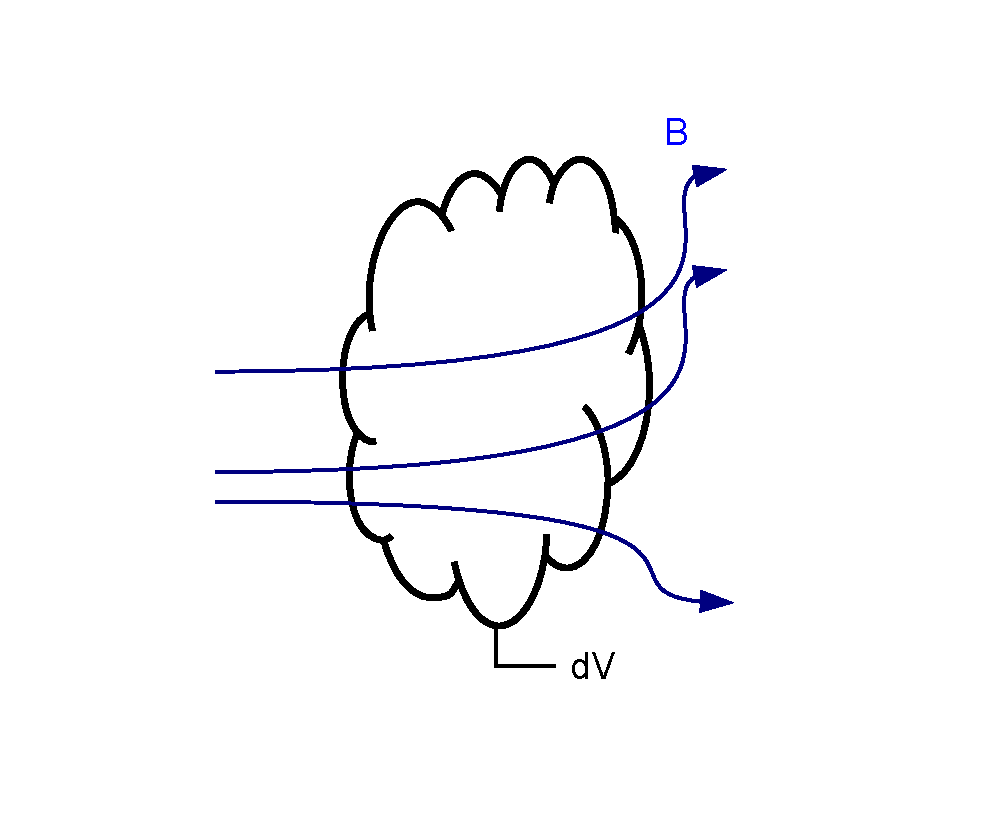
\includegraphics[scale=0.5]{images/maxwell_2.pdf}
\end{center}

\item Wechselnde Induktionsflüsse erzeugen eine Spannung.\\
$ \vec \nabla \times \vec E = - \frac{\partial \vec B}{\partial t} \rightarrow
\oint_{\partial A} \vec E \cdot \vec t ds = - \frac{\partial \Phi}{\partial t}$
\begin{center}
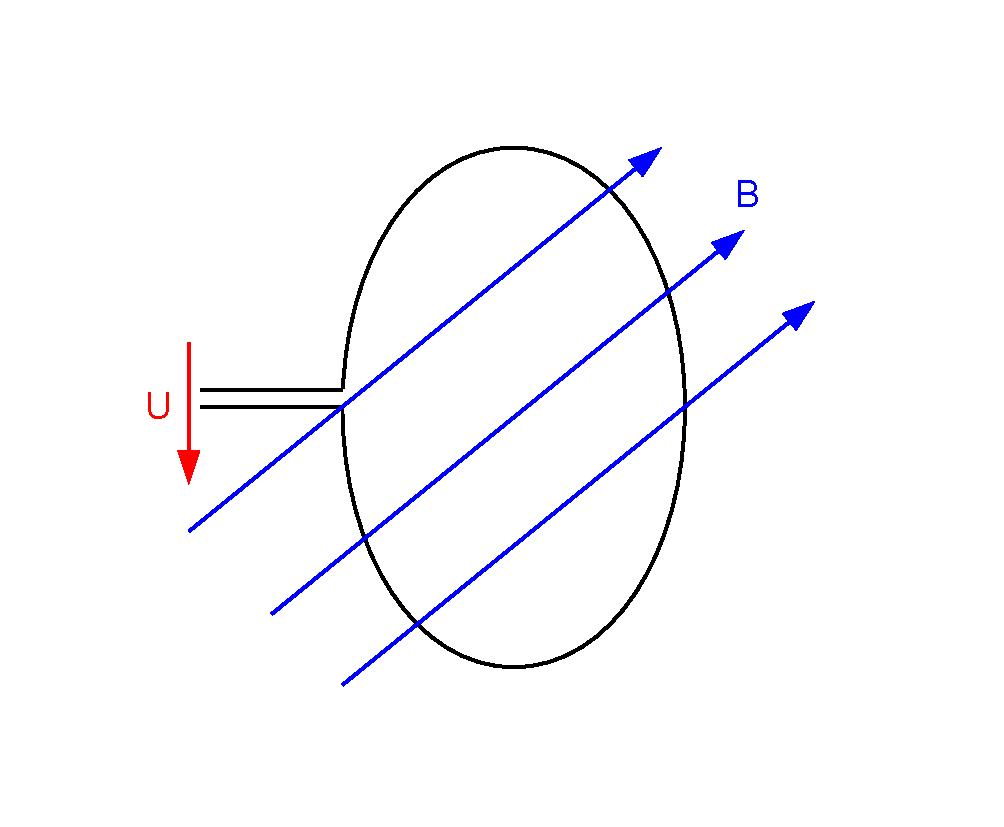
\includegraphics[scale=0.5]{images/maxwell_3.pdf}
\end{center}

\item Magnetische Felder werden durch Sträme (fliessende Ladungen) verursacht
(nur bei kleinen Frequenzen gültig, < 1 GHz)\\
$\vec \nabla \times \vec H = \vec j \rightarrow \oint \vec H \cdot \vec t ds =
I$\\
$I=\int \vec j \vec n dA = \sum I_i$
\begin{center}
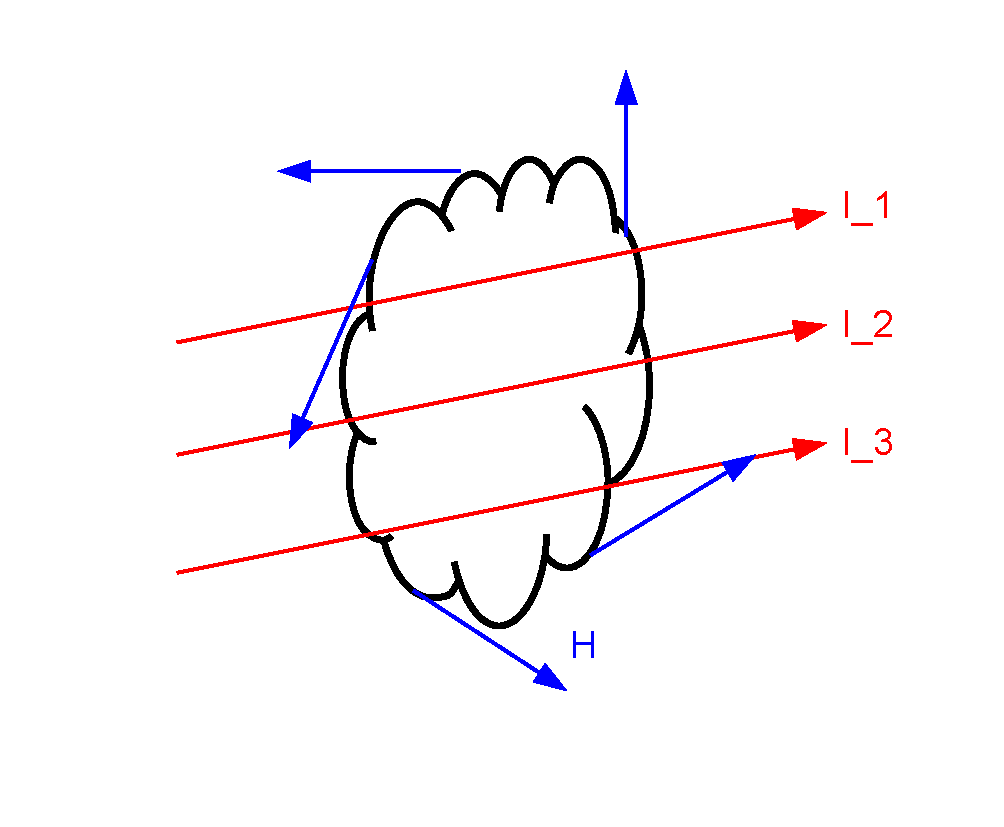
\includegraphics[scale=0.5]{images/maxwell_4.pdf}
\end{center}

\end{itemize}


\section{Wellen}

Kommt nicht ist nicht drin das Kapitelangabe stimmt, juppi

\section{Anhang für Dubeli}
	\subsection{Matrixmultiplikation}
		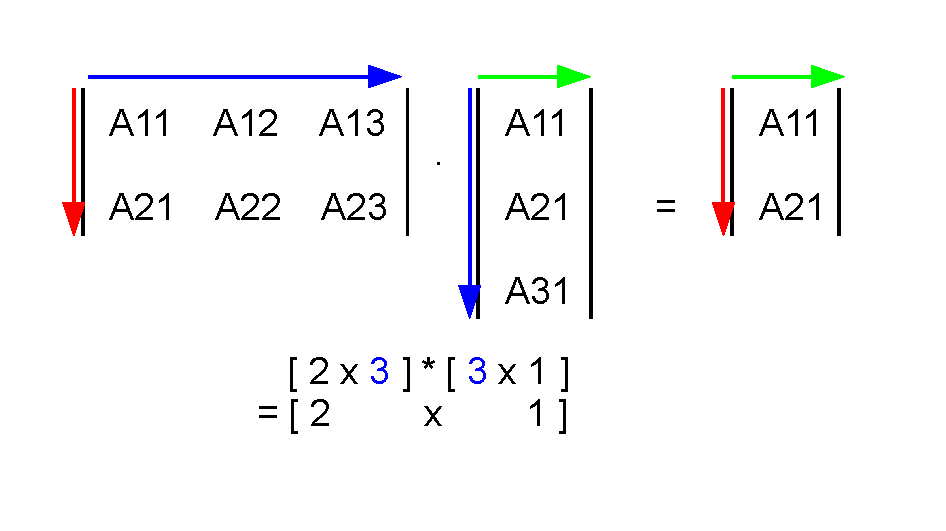
\includegraphics[scale=0.5]{images/matrixmultiplikation.pdf}

	\subsection{Differential-Rechnung}
	  $f'(x_0)=\lim\limits_{\Delta x\rightarrow 0}
	  \frac{f(x_0+\Delta)x-f(x_0)}{\Delta x}$\\
		\begin{tabular}{llll}
			Kettenregel:	& $f\big(g(x)\big)$ &$=$ & $g'(x)\cdot f'\big(g(x)\big)$
			oder $\frac{d f(g(x))}{dx} = f'(g(x)) \cdot g'(x)$\\[0.1cm] Produktregel:	&
			$f(x)\cdot g(x)$ &$=$ & $f'(x)\cdot g(x) + f(x)\cdot g'(x)$\\[0.1cm] Quotientenregel:& $\frac{f(x)}{g(x)}$ &$=$ & $\frac{f'(x)g(x)-f(x)g'(x)}{g^2(x)}$\\
		\end{tabular}
		
		
	\subsection{Taylor Polynom}
		$f(x_0+h)=f(x_0) + f'(x_0)h + \frac{f''(x_0)}{2}h^2 + \frac{f'''(x_0)}{3!}h^3 + \ldots + \frac{f^{(n)}(x_0)}{n!}h^n + R_n(x_0, h)$

	\subsection{Determinanten}
		$\det\left(
		\begin{bmatrix}
			a_{11}&a_{12}\\
			a_{21}&a_{22}\\
		\end{bmatrix}\right)=
		\begin{vmatrix}
			a_{11}&a_{12}\\
			a_{21}&a_{22}\\
		\end{vmatrix}=a_{11}a_{22}-a_{12}a_{21}$
		
	\subsection{Spur}
			$\text{trace}\left(
		\begin{bmatrix}
			a_{11}&a_{12}\\
			a_{21}&a_{22}\\
		\end{bmatrix}\right)=
		a_{11} + a_{22}$\\
		
		\subsection{todo!!!!!!!!!!!!!!}
		\colorbox{red}{Ableitungs und Integral table aus PDE copy, welche
		brauchen wir? stand auf meinem Notizzettel (bischsil)}
		
\section{Glossary}
\begin{itemize}
  \item Orthogonal: $A^T = A^{-1}$
  \item Transponierte Matrix: $A^T = \begin{bmatrix}
  		a_{11}&a_{12}\\
		a_{21}&a_{22}\\
	\end{bmatrix}^T = \begin{bmatrix}
  		a_{11}&a_{21}\\
		a_{12}&a_{22}\\
	\end{bmatrix}$
\end{itemize}


\end{document}


